I doppi - consecutivi dei comandi per via di come Google Documenti
gestisce i simboli sono mostrati come uno singolo, inoltre non è
consigliato copiare direttamente i comandi da qui sulla bash

Docker

Per far partire un container tramite un'immagine (la cerca prima in
locale e poi su Docker Hub), con un nome custom (univoco) e collegarlo
alla rete del Docker host (-d per farlo partire in background
{[}detached mode{]}):

\emph{docker run -d --port portaEsterna:portaInterna --name
nomeContainer nomeImmagine}

\textbf{Oppure}

\textbf{{[}}Non consigliato, perché sappiamo solo la porta
interna\textbf{{]}}

\emph{docker run -d --port portaInterna -- name nomeContainer
nomeImmgina}

\emph{Porta Esterna:} porta del container {[}accedibile da localhost{]}

\emph{Porta Interna:} porta del server {[}data dal container, non è da
cambiare{]}

\textbf{Esempio:}

Se un Docker Engine (PC su cui è installato Docker) contiene un
container che è un server HTTP (nginx) (in esecuzione sulla porta 80), e
vogliamo che dalla rete locale (dove è collegato Docker Engine) si possa
accedere al container devo:

\begin{itemize}
\item
  avere l'indirizzo del Docker Engine;
\item
  avere la porta su dove gira nginx sul Docker Engine (8080)
\end{itemize}

Quindi:

\emph{docker -run -d --port 8080:80 --name miohttp nginx}

Possiamo, dopo aver creato un container, creare un'immagine di esso in
modo da poter \textbf{duplicare velocemente} lo stesso container
{[}Utile all\textquotesingle esame per quando si chiede di creare tanti
nodi{]}:

\emph{docker commit idContainer nomeImmagine}

Successivamente per farlo partire si fanno gli stessi comandi
sopracitati.

\section{Network}\label{network}

\emph{\textbf{{[}MACVLAN non sarà nell'esame{]}}}

Ogni container viene linkato ad una rete {[}\emph{docker network ls}{]}
che di default è \textbf{bridge}; c'è la possibilità di \textbf{creare}
reti custom partendo da modelli base:

\emph{docker network create --driven bridge alpine-net}

Per \textbf{visionare} nel dettaglio ogni rete (bridge in questo caso):

\emph{docker network inspect bridge}

Per esempio è possibile vedere i container al suo interno.

Per \textbf{connettere} un container ad una rete (colleghiamo alpine ad
bridge):

\emph{docker network connect bridge alpine}

Un container può collegarsi a più reti.

Per \textbf{far partire} un container in una rete specifica (host in
questo caso), it serve per interfacciare il nostro container con il
Docker Engine, con una immagine specifica che permette di eseguire un
comando appena fatto partire:

\emph{docker run -it -\/-network=host alpine:latest /bin/ash}

\textbf{Posso anche unire i flag, es: -dit (d per background, it per
interfacciare)}

Questa immagine se non gli si dà un comando all'avvio viene creata e
distrutta subito, perché non ha nessun compito.

Dopo la creazione se vogliamo \textbf{entrare} nel container interattivo
(grazie ad \textbf{-it}) posso usare:

\emph{docker attach alpine}

Ricordarsi di usare \emph{CTRL + P + Q per uscire}.

Se si usa \textbf{exit} o \textbf{CTRL+D} l'interprete dei comandi si
spegne e così il container.

\section{Mantenere stato}\label{mantenere-stato}

\subsection{Bind mount}\label{bind-mount}

Collega una cartella/file della nostra macchina (Docker Engine) nel
container.

Per fare mount di una cartella dalla nostra macchina sul container:

\emph{docker run -dit -v \textbf{/percorso/macchina:/percorso/container}
alpine:latest /bin/ash}

\textbf{Esempio:}

\emph{docker run -dit -v
C:\textbackslash Users\textbackslash matte\textbackslash Desktop\textbackslash prova:/tmp
alpine:latest /bin/ash}

\emph{\textbf{RIcordarsi di mettere ``\,'' se il percorso ha spazi}}

Ora da dentro il container in /tmp sarà possibile accedere alla cartella
\textbackslash prova e ai suoi file.

\subsection{Volume}\label{volume}

Salva sempre le cartelle/file su un'area della nostra macchina ma è
gestito completamente da Docker ed hanno un ciclo di vita al di fuori e
non dipendente dal container.

Per \textbf{usare} un volume:

\emph{docker run -dit -v \textbf{nomeVolume:/percorso/container}
alpine:latest /bin/ash}

\textbf{Esempio:}

\emph{docker run -dit -v volumeEsempio:/tmp alpine:latest /bin/ash}

Sostanzialmente se non si mette un path specifico crea un volume con
quel nome, possiamo \textbf{vedere} i volumi creati con:

\emph{docker volume ls}

e per vederli nel \textbf{dettaglio}:

\emph{docker volume inspect nomeVolume}

Per \textbf{eliminare} i container che non usano volumi facciamo:

\emph{docker volume prune}

Jenkins

Automation server per creare delle pipeline in fase di sviluppo, in modo
da automatizzare processi che vengono fatti in maniera ripetuta.

Per scaricare l'immagine di jenkins e la chiamiamo jenkinsMaster:

\emph{docker run -\/-name jenkinsMaster -p 8080:8080 -p 50000:50000 -d
-v jenkins\_home:/var/jenkins\_home jenkins/jenkins}

Successivamente possiamo ottenere la password per accedere all'account
admin tramite {[}da fare dopo averli fatto partire{]}:

\emph{docker logs nomeContainer}

\section{Pipeline}\label{pipeline}

La sintassi per le pipeline è:

pipeline \{

agent any

stages \{

stage(\textquotesingle Stage 1\textquotesingle) \{

steps \{

echo \textquotesingle Hello world!\textquotesingle{}

\}

\}

\}

\}

Dove \emph{any}, indica in quali nodi eseguire la pipeline, in questo
caso tutti.

\subsection{Git}\label{git}

Per avviare uno script residente su GitHub possiamo seguire i seguenti
passaggi:

\begin{enumerate}
\def\labelenumi{\arabic{enumi}.}
\item
  Andiamo nella pagina di creazione;
\item
  Cliccare: \textbf{Pipeline Syntax}, collocato sotto la sezione di
  inserimento della pipeline.
\item
  In \emph{Sample Step} mettere \textbf{git: Git}.
\item
  Inserire l'URL, il nome del ramo e le credenziali.
\item
  Generare la pipeline e copiarla.
\item
  Creare uno script con diversi stage, uno con il comando copiato e uno
  per avviare il file.
\end{enumerate}

Esempio:

pipeline \{

agent any

stages \{

stage(\textquotesingle inizio\textquotesingle) \{

steps \{

echo \textquotesingle pipeline avviata correttamente\textquotesingle{}

\}

\}

stage(\textquotesingle fetch\textquotesingle) \{

steps \{

git branch: \textquotesingle main\textquotesingle, credentialsId:
\textquotesingle c6d7c2d5-8649-4650-981c-c6b80e94d27e\textquotesingle,
url:
\textquotesingle https://github.com/scastagnoli/PythonDevOps.git\textquotesingle{}

\}

\}

stage(\textquotesingle esecuzione\textquotesingle) \{

steps \{

sh \textquotesingle python3 liste.py\textquotesingle{}

\}

\}

\}

\}

\subsection{Triggered pipeline}\label{triggered-pipeline}

Esistono due modalità:

\begin{itemize}
\item
  \textbf{cron}: come il daemon dentro Linux permette di eseguire la
  pipeline ad intervalli regolari;
\item
  \textbf{pollSCM}: la pipeline controlla dal sorgente SCM (git o altro)
  se ci sono modifiche, in caso viene eseguita.
\end{itemize}

\emph{La pipeline deve essere \textbf{eseguita manualmente una volta}
prima che il trigger venga preso in considerazione !!!}

\textbf{Struttura generale:}

pipeline \{

agent any

triggers \{

cron(\textquotesingle H * */4 * * 1-5\textquotesingle)

\}

stages \{

\begin{quote}
stage(\textquotesingle Example\textquotesingle) \{

steps \{

echo \textquotesingle Hello World\textquotesingle{}

\}

\}
\end{quote}

\}

\}

L'\textbf{H} indica un hash della pipeline corrente, che rende
leggermente casuale l'esecuzione, così anche se ci sono tante pipeline
che vengono eseguite con gli stessi intervalli evita conflitti.

Esempi di trigger:

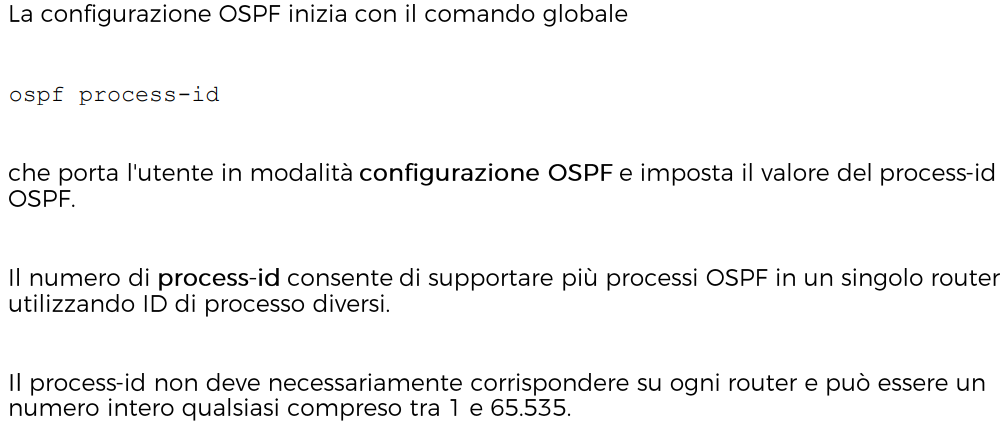
\includegraphics[width=6.26772in,height=2.18056in]{media/image4.png}

\emph{Si può controllare se la combinazione è giusta qui:
\href{https://crontab.guru/}{\ul{https://crontab.guru/}}}

\section{Master-Slave}\label{master-slave}

Dopo aver creato un nuovo nodo in \emph{Permanent Node} (Gestisci
Jenkins -\textgreater{} Nodes -\textgreater{} New Node -\textgreater{}
nome nodo e mode) e aver impostato l'ind. IP per URL di Jenkins
(dashboard-\textgreater gestisci
Jenkins-\textgreater System-\textgreater URL di Jenkins) possiamo creare
un container che ospiterà il nostro slave e scaricare al suo interno jdk
(per compilare java), curl e git:

\begin{quote}
\emph{•docker run -dit -\/-name nomeSlave debian}

\emph{•docker exec -it nomeSlave /bin/bash}

\emph{•apt update}

\emph{•apt install default-jdk curl git}
\end{quote}

Questo container funge da nodo slave.

Per connettersi a Jenkins eseguiamo i comandi che prendiamo dalla pagina
del nodo direttamente da Jenkins.

Se tutto va come previsto nella bash dovrebbe uscire:

\emph{INFO: Connected}

e come prova del nove se andiamo sulla pagina dei nodi in Jenkins
notiamo che dice connesso e l'icona non è barrata.

In caso il nodo debba essere connesso nuovamente rifare i comandi dati
da Jenkins (in particolare quello java con l'indirizzo ip).

Ora possiamo eseguire pipeline sui diversi nodi slave, mettendo
\emph{negli agent i nomi di Jenkins} \textbf{e NON} quello del
container.

Ansible

Permette di centralizzare e automatizzare la gestione e i processi su
dei nodi e il controllo del loro stato.

Gli elementi fondamentali di questa tecnologia sono:

\begin{itemize}
\item
  \textbf{Control node}: nodo dove vengono eseguiti i comandi per
  controllare gli altri nodi.

  \begin{itemize}
  \item
    \textbf{Inventory}: elenco dei nodi controllati, sta nel nodo di
    controllo.
  \end{itemize}
\item
  \textbf{Managed node}: nodi controllati dal Control node
\end{itemize}

\emph{\textbf{Da ricordare}: il Control Node NON è un server, anzi è lui
che si collegherà ai vari nodi !!!}

\section{Configurazione nodi/ssh}\label{configurazione-nodissh}

Per preparare i nodi:

\begin{itemize}
\item
  \emph{docker run -dit --name nomeNodo debian}
\item
  \emph{apt update} {[}Dentro al container, per entrare usa \emph{docker
  exec -it nome bash}{]}
\item
  \emph{apt install python3 openssh-server nano ansible}
\end{itemize}

\begin{quote}
\emph{Solo sul nodo di controllo (Control node)}
\end{quote}

Successivamente vanno generate le key pair (dentro al Control Node), la
chiave privata rimarrà nel nodo di controllo e i managed node avranno
quella pubblica:

\begin{itemize}
\item
  \textbf{{[}Control Node{]}} \emph{ssh-keygen}: successivamente verrà
  chiesto -\textgreater{}

  \begin{itemize}
  \item
    \textbf{nome:} \emph{/root/.ssh/nomeFile};
  \item
    \textbf{passphrase (da ricordare):} \emph{password}.
  \end{itemize}
\end{itemize}

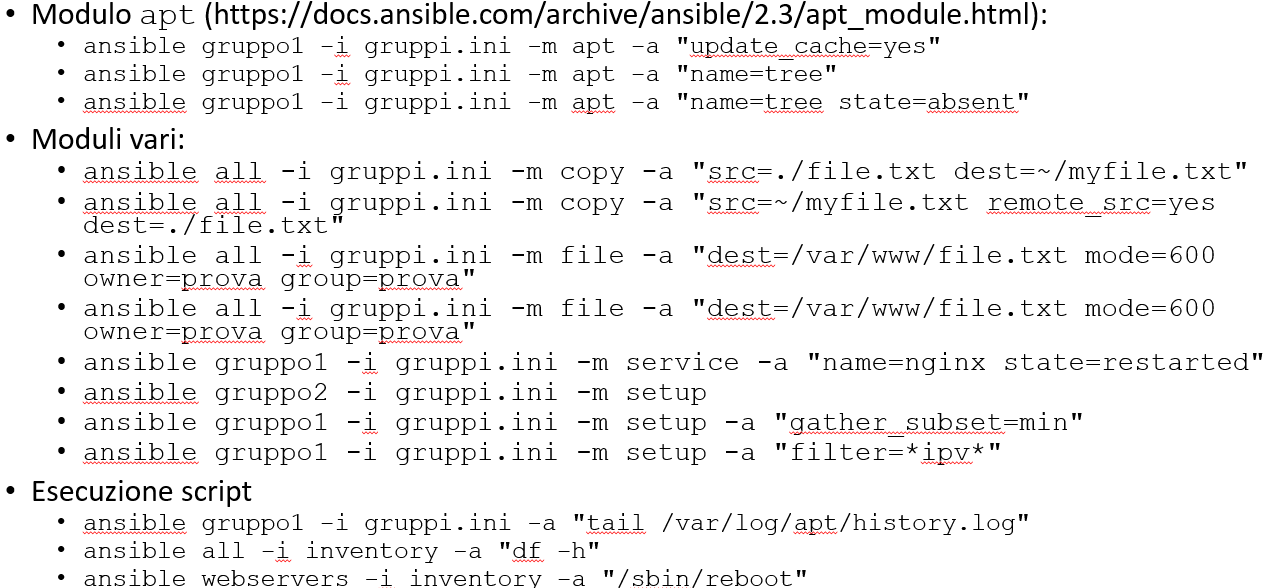
\includegraphics[width=4.06384in,height=2.25521in]{media/image2.png}

Per salvare la passphrase per evitare che venga chiesta ad ogni
connessione \textbf{{[}Facoltativo{]} {[}Control Node{]}}:

\begin{itemize}
\item
  \emph{exec ssh-agent \$SHELL}
\item
  \emph{ssh-add /root/.ssh/nomeFile}
\item
  \textbf{{[}Comando di verifica{]}} \emph{ssh-add -l}
\end{itemize}

Ora bisogna distribuire la chiave pubblica ai Managed node, per farlo
dobbiamo modificare il file di configurazione di ssh :

\begin{itemize}
\item
  \textbf{{[}Managed Node{]}} \emph{nano /etc/ssh/sshd\_config}: e
  modifichiamo le seguenti voci (cercale con CTRL + W):

  \begin{itemize}
  \item
    \textbf{PermitRootLogin yes}
  \item
    \textbf{PubkeyAuthentication yes}
  \item
    \textbf{AuthorizedKeysFile .ssh/nomeFile.pub} {[}ricordarsi di
    prendere la chiave dal control node (cat root/.ssh/nomeFile.pub),
    copiarla, e inserirla nel file in questa posizione{]}
  \item
    \textbf{PasswordAuthentication no}
  \end{itemize}
\end{itemize}

Per poi \textbf{restartare} il server ssh \textbf{{[}Managed Node{]}}:

\begin{itemize}
\item
  \emph{/etc/init.d/ssh restart}
\item
  \emph{/etc/init.d/ssh status}
\end{itemize}

Per verificare l'accessibilità dei nodi va fatto:

\begin{itemize}
\item
  \textbf{{[}Control Node{]}} \emph{ssh -i /root/.ssh/nomeFile
  root@host}
\end{itemize}

\begin{quote}
\emph{Si prende facendo \textbf{docker inspect bridge nomeContainer} sul
Docker Engine (IP Address)}
\end{quote}

\textbf{NOTA BENE:} se si decide di usare docker commit, per duplicare i
nodi velocemente, usare il comando:

\emph{ssh-keygen -q -N ``\,'' -t ed25519 -f
/etc/ssh/ssh\_host\_ed25519\_key}

in modo da generare un nuovo fingerprint per il server ssh (ricordarsi
di fare il restart).

Altrimenti ssh non riuscirà a connettersi al host duplicato perché è
settato per evitare un attacco di tipo Man in The Middle.

\section{Funzionamento}\label{funzionamento}

Ora che abbiamo creato i container e configurato SSH possiamo passare ad
usare \textbf{Ansible}.

Per iniziare bisogna creare l'\textbf{inventory}, quindi dentro il
Control Node creiamo un file .ini dove inseriamo i gruppi con ciascun
nodo, esempio:

{[}gruppo1{]}

172.17.0.4

172.17.0.5

{[}gruppo2{]}

172.17.0.7

{[}vm{]}

192.168.178.123

Possiamo vedere come sia possibile inserire anche VM oltre che host (non
è necessario).

Successivamente è possibile fare diversi comandi di Ansible, esempio:

\begin{itemize}
\item
  \emph{ansible gruppo1 -m ping -i gruppi.ini} =\textgreater{} dove
  faccio ping a tutti i nodi del gruppo 1, prendendo le informazioni dal
  file gruppo.ini.
\end{itemize}

Esistono diversi pattern per far eseguire i comandi a diversi nodi:


\includegraphics[width=6.27083in,height=1.45147in]{media/image1.png}

In generale un comando \textbf{Ansible} è così strutturato:

\emph{ansible \textbf{target} -i \textbf{inventory} {[}-m
\textbf{module} {[}-a \textbf{``module options''}{]}{]}}

Dove:

\begin{itemize}
\item
  \textbf{target}: i nodi destinatari del comando;
\item
  \textbf{inventory}: il file da dove prendere i target/gruppi/ecc;
\item
  \textbf{module}: nome del modulo da usare (il comando);
\item
  \textbf{module options}: dipende dal comando usato, se non uso
  \emph{-m} posso inserire uno script da usare.
\end{itemize}

Ecco alcuni esempi:


\includegraphics[width=6.26772in,height=2.88889in]{media/image3.png}

\subsection{Playbook}\label{playbook}

Servono per eseguire comandi Ansible in modo semplice e flessibile.

I due formati sono:

\begin{itemize}
\item
  .ini: semplici ma meno flessibili;
\item
  .yaml: usati praticamente sempre quando la complessità aumenta.
\end{itemize}

Esempio di sintassi, ricordarsi che è necessario rispettare gli spazi:


\includegraphics[width=6.26772in,height=2.98611in]{media/image5.png}

Si possono avviare con il comando:

\emph{ansible-playbook -i inventory.ini nomeFile.yaml}

Creare un VM con docker:
\href{https://secgroup.dais.unive.it/teaching/vm-with-docker/}{\ul{https://secgroup.dais.unive.it/teaching/vm-with-docker/}}

Kubernetes

Sistema di orchestrazione di container. Composto da Nodi (macchina che
esegue attività), cluster (nodi logicamente correlati), pod (uno o più
container distribuiti su un singolo nodo, con stesso IP, IPC, nome host
ecc)) e Control plane (controlla i nodi e i cluster).

\section{Set up}\label{set-up}

Per vedere come creare e settare la macchina virtuale:
\href{https://unibo.cloud.panopto.eu/Panopto/Pages/Viewer.aspx?id=c51d7154-78e0-4816-a740-b22600f9d90f}{\ul{https://unibo.cloud.panopto.eu/Panopto/Pages/Viewer.aspx?id=c51d7154-78e0-4816-a740-b22600f9d90f}}

\section{Comandi}\label{comandi}

Per creare un namespace:

\emph{kubectl create namespace nomeNamespace}

Visualizzare i namespace;

\emph{kubectl get namespace}

Creare dei deployment di un'immagine in un namespace specifico:

\emph{kubectl create deployment nomeDeploy --image=nomeImage
-n=nomeNamespace}

Visualizzare i deployment di un namespace:

\emph{kubectl get deployment -n nomeNamespace}

Visualizzare tutti i deployment di tutti i namespace:

\emph{kubectl get deployment -A}

Cambiare namespace corrente:

\emph{kubectl config set-context - -current - -namespace=nomeNamespace}

per assicurarsi di essere nel giusto:

\emph{kubectl config get-contexts}

Ottenere informazioni su un deployment {[}\textbf{DA FARE DENTRO IL
RISPETTIVO NAMESPACE}{]}:

\emph{kubectl describe deployment nomeDeploy}

Visualizzare il log di un deployment, utile in caso di errore
{[}\textbf{DA FARE DENTRO IL RISPETTIVO NAMESPACE}{]}:

\emph{kubectl logs deployment/nomeDeploy}

Cancellare tutti i deployment di un namespace:

\emph{kubectl delete deployment --all -n nomeNamespace}

Visualizzare in quali nodi sono in esecuzione i pods:

\emph{kubectl get pods -o wide}

MQTT
